\documentclass[12pt,a4paper]{article}

\usepackage[a4paper,margin=1in]{geometry}
\usepackage[T1]{fontenc}
\usepackage[utf8]{inputenc}
\usepackage{lmodern}
\usepackage{array}
\usepackage{booktabs}
\usepackage{tabularx}
\usepackage{longtable}
\usepackage{graphicx}
\usepackage{xcolor}
\usepackage{float}
\usepackage{caption}
\usepackage{subcaption}
\usepackage{fancyhdr}
\usepackage{hyperref}
\usepackage{xurl}
\usepackage{listings}
\usepackage{tikz}
\usepackage{enumitem}
\usepackage{titlesec}
\usepackage{setspace}
\usepackage{ragged2e}
\usepackage{parskip}
\usepackage{pdflscape}
\usetikzlibrary{arrows.meta,positioning,fit,calc}

\graphicspath{{figures/}}
\hypersetup{
    colorlinks=true,
    linkcolor=blue,
    urlcolor=blue,
    pdftitle={Hopper Project Report},
    pdfauthor={Four-Eyed Raven}
}

\definecolor{todored}{RGB}{180,0,0}
\newcommand{\todo}[1]{\textcolor{todored}{TODO: #1}}

\lstdefinestyle{hoppercode}{
    basicstyle=\ttfamily\small,
    breaklines=true,
    frame=single,
    columns=fullflexible,
    keepspaces=true
}
\lstset{style=hoppercode}

\pagestyle{fancy}
\fancyhf{}
\lhead{Hopper}
\rhead{Internet Programming Lab Report}
\cfoot{\thepage}
\setlength{\headheight}{14.5pt}
\setstretch{1.15}

\titleformat{\section}{\large\bfseries}{\thesection.}{0.5em}{}
\titleformat{\subsection}{\normalsize\bfseries}{\thesubsection}{0.5em}{}

\begin{document}
\pagenumbering{gobble}

\begin{titlepage}
    \centering
    \vspace*{1.5cm}

    {\Large \textbf{CSE 4113 -- Internet Programming Lab}\par}
    \vspace{1cm}
    {\LARGE \textbf{Project Report}\par}
    \vspace{1.25cm}
    {\Huge \textbf{Hopper}\par}
    \vspace{0.5cm}
    {\Large \textbf{Team: Four-Eyed Raven}\par}
    \vspace{1.25cm}

    {\large \textbf{Submitted By}\par}
    \vspace{0.5cm}

    \renewcommand{\arraystretch}{1.35}
    \begin{tabularx}{\textwidth}{|>{\RaggedRight\arraybackslash}X|>{\RaggedRight\arraybackslash}X|}
        \hline
        \textbf{Team Member} & \textbf{Student ID} \\
        \hline
        \todo{Add member 1 name} & \todo{Add student ID} \\
        \hline
        \todo{Add member 2 name} & \todo{Add student ID} \\
        \hline
        \todo{Add member 3 name} & \todo{Add student ID} \\
        \hline
        \todo{Add member 4 name} & \todo{Add student ID} \\
        \hline
    \end{tabularx}

    \vfill

    {\large \textbf{\todo{Add batch information}}\par}
    \vspace{0.25cm}
    {\large Department of Computer Science \& Engineering\par}
    {\large University of Dhaka\par}
    \vspace{0.75cm}
    {\large \textbf{Submitted On}\par}
    {\large 23.07.2026\par}
\end{titlepage}

\clearpage
\pagenumbering{arabic}
\tableofcontents
\newpage

\section*{Project Links}
\addcontentsline{toc}{section}{Project Links}

\begin{tabularx}{\textwidth}{|>{\RaggedRight\arraybackslash}p{0.34\textwidth}|>{\RaggedRight\arraybackslash}X|}
    \hline
    \textbf{Item} & \textbf{URL} \\
    \hline
    Public Git Repository & \url{https://github.com/CREVIOS/Hopper} \\
    \hline
    Deployed Application URL & \url{https://hopper.farefin.com} \\
    \hline
    API Docs (Swagger/Postman) -- public link & \url{https://hopper.farefin.com/api/docs} \\
    \hline
    Demo Video & \todo{Add public demo video URL} \\
    \hline
\end{tabularx}

\newpage

\section{Introduction}
\subsection{Problem Definition \& Context}
Hopper is a self-hosted compute provisioning platform intended for university environments. The repository describes it as a system that slices institution-owned bare-metal resources into isolated runtime environments that can be requested through a web interface, accessed over SSH, and governed through credit-based usage control and single sign-on integration. In the current implementation, the platform exposes these runtimes as Kubernetes-backed pod sessions while preserving the user-facing concept of provisioned virtual machine style workspaces.

The codebase shows that the project addresses several operational problems at once. First, shared academic compute infrastructure requires stronger isolation than ad hoc account sharing or manually provisioned hosts. Second, institutions need a practical way to manage fair usage, including per-session billing and automatic shutdown when credits are exhausted. Third, a university deployment must integrate with centralized identity management rather than maintaining a separate manual authentication system. Hopper therefore combines a browser-based control plane, an API layer, an orchestration service, a relational ledger-backed data model, and Keycloak-based authentication in one deployable platform.

\subsection{Target Users \& Use Cases}
The verified user model in the repository includes at least three application roles: student, professor, and admin. These roles appear in the documented Keycloak realm configuration and are reflected in frontend routes and backend authorization logic. The system therefore serves both end users who consume compute sessions and privileged users who supervise access, credits, and platform status.

Students are the primary runtime users. Confirmed use cases include signing in through the authentication flow, viewing available plans, creating and terminating compute sessions, monitoring CPU and memory usage, opening browser-based development access, using SSH-related settings, and reviewing their credit balance and usage history. Professors and administrators have additional operational and oversight use cases, including allocating credits, inspecting node or platform statistics, reviewing users, and accessing administrative workflows exposed through dedicated backend and frontend routes.

\subsection{Core Features}
The repository confirms that Hopper provides a multi-service compute management workflow rather than a static informational website. Core platform features include authenticated session management through Keycloak, plan-based runtime creation, automated credit checks before provisioning, orchestration of pod lifecycle events through a Go service, and persistent tracking of sessions and ledger operations in PostgreSQL with TimescaleDB support. These features are reinforced by the documented API routes, backend services, database migrations, and deployment manifests.

The frontend and backend code also confirm several user-facing capabilities beyond simple provisioning. The platform includes real-time metrics delivery through Server-Sent Events, browser-based terminal and file-management related functionality, administrative dashboards, SSH key management, notifications, and issue-reporting support. The infrastructure and documentation further show support for ingress-based web delivery, TLS termination, Keycloak-backed login and logout, NATS-based event propagation for billing and lifecycle messages, and Kubernetes deployment resources for a full cluster-based installation.

\subsection{Tech Stack Overview}
The frontend is implemented with SvelteKit 2, Svelte 5, TypeScript, and Vite. This choice is suitable because the project needs route-driven server rendering, interactive dashboards, and a structured component model for authenticated application pages. The dependency set and source tree also show use of lightweight Svelte stores and derived state rather than a heavyweight external state library. In practice, state management is handled through Svelte writable stores for concerns such as authentication, pod state, and notifications, together with route-level server load functions and local derived state in components.

The backend is implemented as a FastAPI application in Python 3.12, backed by Pydantic settings, SQLAlchemy, Alembic migrations, and supporting libraries for SSE, authentication, rate limiting, and asynchronous I/O. This stack is suitable because it supports typed API development, automatic OpenAPI documentation, asynchronous integration with external services, and relatively clear separation of routers, services, models, and middleware. The repository also contains a Go 1.23 orchestration service that uses gRPC and Kubernetes client libraries, which is appropriate for cluster-facing lifecycle management because the native Kubernetes tooling in Go is mature and directly aligned with the platform's orchestration requirements.

The primary database layer is PostgreSQL with TimescaleDB. This combination is suitable because Hopper needs conventional relational storage for users, sessions, roles, and accounting data, while also benefiting from time-series capabilities for metrics aggregation. Messaging and event distribution are handled through NATS JetStream, which fits the platform's need for lightweight asynchronous communication between the orchestrator and the API gateway, especially for billing and metrics events. Authentication is provided by Keycloak using OIDC flows, which is suitable for institutional single sign-on integration and role-based access control.

The deployment and hosting configuration is centered on Kubernetes, Nginx Ingress, and declarative infrastructure artifacts under \texttt{k8s/}, \texttt{charts/}, and \texttt{infrastructure/}. This is suitable because the platform provisions compute sessions as cluster workloads and depends on ingress routing, service discovery, and namespace-level policy enforcement. The repository also confirms supporting infrastructure such as Docker and Docker Compose for local services, cert-manager for TLS certificate automation, and Cilium-enforced network policy definitions for zero-trust traffic control. Optional outbound email support is configured through Brevo or SMTP, but the exact production mail configuration remains environment-dependent.

\section{System Architecture}
\subsection{High-Level Architecture Diagram}
The deployed system is organized as a browser-facing frontend, a Python API gateway, a Go orchestration service, an identity provider, a relational database layer, and an event bus. The ingress configuration under \texttt{k8s/deploy/03-ingress.yaml} shows that external traffic is split across four path families: \texttt{/} for the frontend, \texttt{/api} for the gateway, Keycloak realm/resource paths for authentication, and a dedicated code-server proxy path for browser-based development access. The API gateway then coordinates synchronous database work, gRPC calls to the orchestrator, and asynchronous event handling over NATS.

At runtime, the orchestrator is the component that directly manages Kubernetes resources. The FastAPI gateway does not create pods itself; instead it creates or updates the application-facing database state, invokes the orchestrator over gRPC, and consumes follow-up events such as billing, pod lifecycle changes, and metrics updates. PostgreSQL stores the authoritative relational state for users, sessions, the credit ledger, notifications, queue entries, and other application records, while TimescaleDB features are used where available for metrics retention and hypertable support.

\begin{figure}[H]
    \centering
    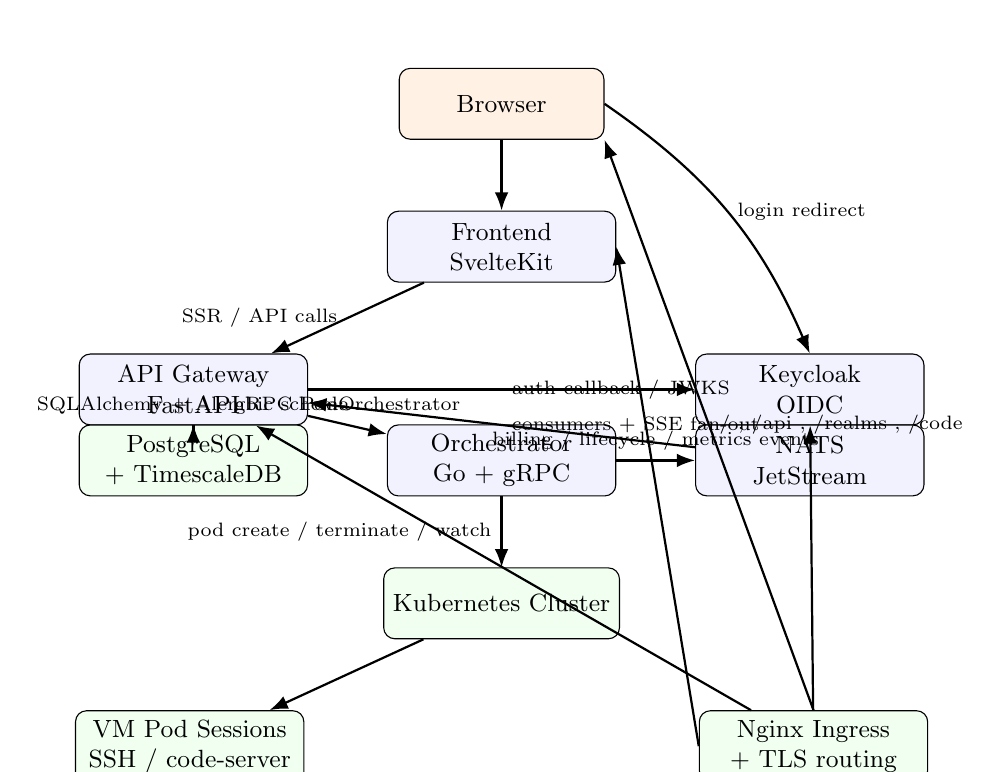
\begin{tikzpicture}[
    font=\small,
    >=Latex,
    node distance=9mm and 10mm,
    service/.style={draw, rounded corners, align=center, minimum width=29mm, minimum height=9mm, fill=blue!5},
    infra/.style={draw, rounded corners, align=center, minimum width=29mm, minimum height=9mm, fill=green!6},
    ext/.style={draw, rounded corners, align=center, minimum width=26mm, minimum height=9mm, fill=orange!10},
    flow/.style={->, thick}
]
\node[ext] (browser) {Browser};
\node[service, below=of browser] (frontend) {Frontend\\SvelteKit};
\node[service, below left=of frontend] (api) {API Gateway\\FastAPI};
\node[service, below right=of frontend] (keycloak) {Keycloak\\OIDC};
\node[service, below=18mm of frontend] (orch) {Orchestrator\\Go + gRPC};
\node[service, right=of orch] (nats) {NATS\\JetStream};
\node[infra, left=of orch] (db) {PostgreSQL\\+ TimescaleDB};
\node[infra, below=of orch] (k8s) {Kubernetes Cluster};
\node[infra, below left=of k8s] (pods) {VM Pod Sessions\\SSH / code-server};
\node[infra, below right=of k8s] (ingress) {Nginx Ingress\\+ TLS routing};

\draw[flow] (browser) -- (frontend);
\draw[flow] (browser.east) to[bend left=16] node[right, font=\scriptsize] {login redirect} (keycloak.north);
\draw[flow] (frontend) -- node[left, font=\scriptsize] {SSR / API calls} (api);
\draw[flow] (api) -- node[above, font=\scriptsize] {SQLAlchemy + Alembic schema} (db);
\draw[flow] (api) -- node[above, font=\scriptsize] {gRPC PodOrchestrator} (orch);
\draw[flow] (api) -- node[right, font=\scriptsize] {auth callback / JWKS} (keycloak);
\draw[flow] (orch) -- node[above, font=\scriptsize] {billing / lifecycle / metrics events} (nats);
\draw[flow] (nats) -- node[right, font=\scriptsize] {consumers + SSE fan-out} (api);
\draw[flow] (orch) -- node[left, font=\scriptsize] {pod create / terminate / watch} (k8s);
\draw[flow] (k8s) -- (pods);
\draw[flow] (ingress.north) -- node[right, font=\scriptsize] {/ , /api , /realms , /code} (browser.south east);
\draw[flow] (ingress.west) -- (frontend.east);
\draw[flow] (ingress) -- (api);
\draw[flow] (ingress) -- (keycloak);
\end{tikzpicture}

    \caption{Verified high-level Hopper architecture derived from the frontend, gateway, orchestrator, and Kubernetes deployment files.}
    \label{fig:hopper-high-level-architecture}
\end{figure}

Figure~\ref{fig:hopper-high-level-architecture} reflects the concrete implementation rather than an aspirational design. In particular, the current repository confirms the following communication paths: browser-to-frontend delivery over ingress, frontend-to-gateway HTTP calls, gateway-to-orchestrator gRPC calls, orchestrator-to-Kubernetes lifecycle control, orchestrator-to-NATS event publication, gateway-side NATS consumers for billing and metrics, and Keycloak-mediated authentication with cookie-backed application sessions.

\begin{figure}[H]
    \centering
    % Figure 2 — Main request and data flow
% Layout (3 rows × 4 columns, all positions in cm):
%
%   Row 0  y= 0.0 : Browser(0) | SvelteKit(4) | API Gateway(8) | Orchestrator(12.5)
%   Row 1  y=-3.0 :             |               | PostgreSQL(8)  | NATS(12.5)
%   Row 2  y=-6.0 :             |               |                | Kubernetes(12.5)
%
% Strict separation rules:
%   • API  south  (x=8.0)   → only arrow 5 (API→DB), shifted slightly left
%   • API  south  (x=8.0)   → arrow 10 (SSH) exits below DB on a far-left rail
%   • Orch south east (x=12.5) split: arrow 6 exits east side → NATS south,
%                                     arrow 9 exits south → K8s north
%   • SSE (11) and WS (12) return paths run above row 0 so nothing crosses boxes
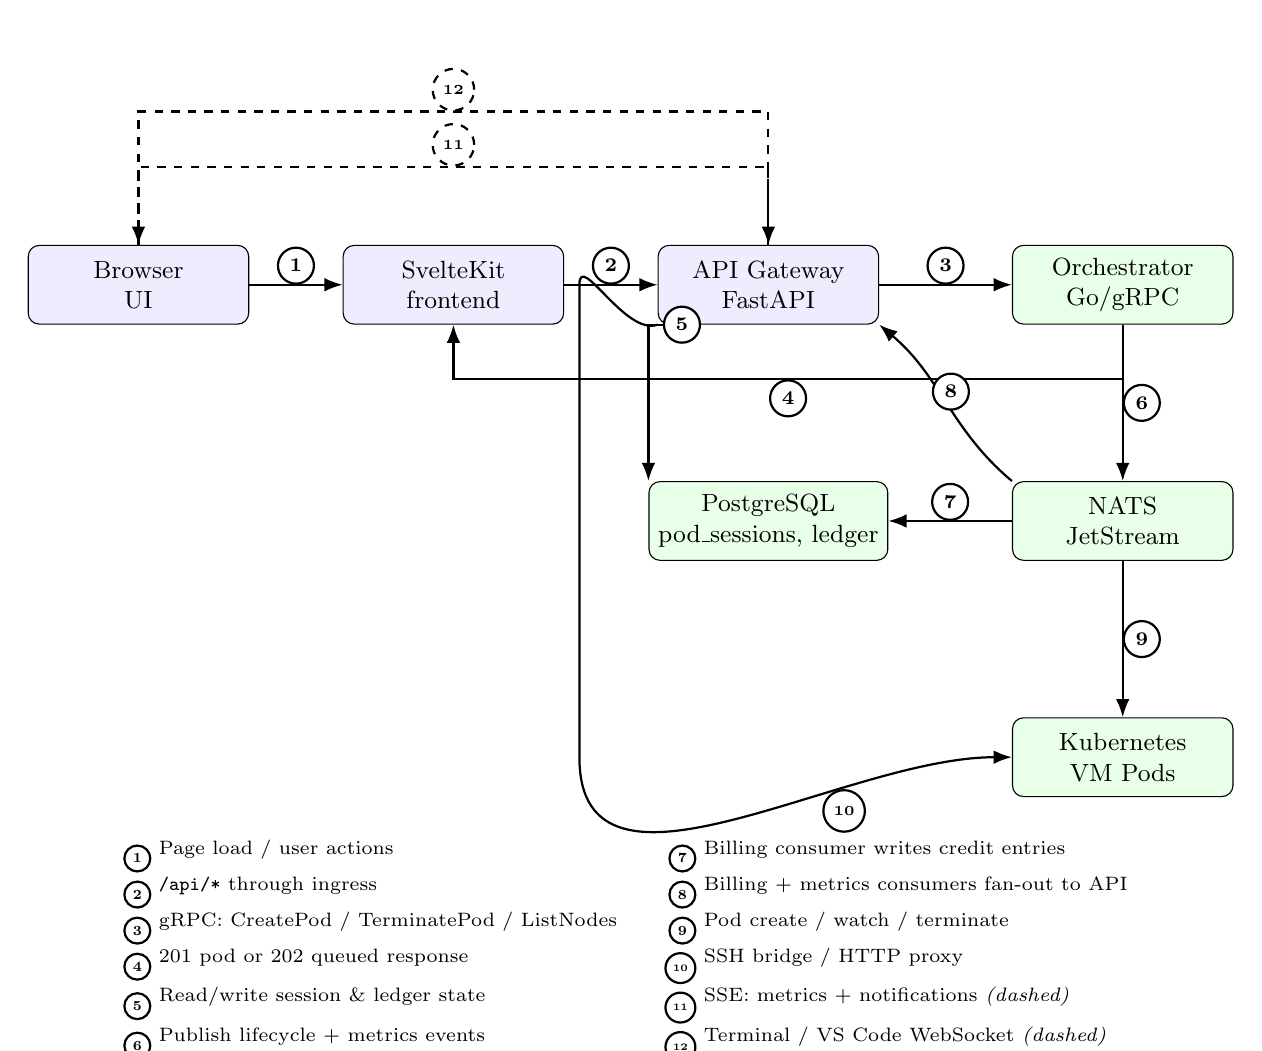
\begin{tikzpicture}[
    font=\small,
    >=Latex,
    box/.style={draw, rounded corners=4pt, align=center,
                minimum width=28mm, minimum height=10mm, fill=blue!7},
    data/.style={draw, rounded corners=4pt, align=center,
                 minimum width=28mm, minimum height=10mm, fill=green!9},
    arr/.style={->, thick},
    das/.style={->, thick, dashed},
    lbl/.style={font=\scriptsize, inner sep=1.5pt,
                fill=white, rounded corners=2pt},
    % Single-digit step marker: circle sized for one character
    stepS/.style={circle, draw, thick, fill=white,
                  font=\scriptsize\bfseries,
                  inner sep=1.2pt, minimum size=13pt},
    % Double-digit step marker: slightly wider circle sized for two characters
    stepD/.style={circle, draw, thick, fill=white,
                  font=\tiny\bfseries,
                  inner sep=0.8pt, minimum size=15pt},
]

%% ── Convenience command: inline circle node on an arrow ─────────────────────
%% Usage:  \stepnode{style}{number}
%% Drop one of these with node[stepS]{1} or node[stepD]{10} in draw paths.

%% ── Node placement ──────────────────────────────────────────────────────────
\node[box]  (ui)   at ( 0.0,  0.0) {Browser\\UI};
\node[box]  (fe)   at ( 4.0,  0.0) {SvelteKit\\frontend};
\node[box]  (api)  at ( 8.0,  0.0) {API Gateway\\FastAPI};
\node[data] (orch) at (12.5,  0.0) {Orchestrator\\Go/gRPC};
\node[data] (db)   at ( 8.0, -3.0) {PostgreSQL\\pod\_sessions, ledger};
\node[data] (nats) at (12.5, -3.0) {NATS\\JetStream};
\node[data] (k8s)  at (12.5, -6.0) {Kubernetes\\VM Pods};

%% ── Arrow 1 : Browser → SvelteKit (page load / user actions) ───────────────
\draw[arr] (ui.east)
    -- node[stepS, above] {1}
    (fe.west);

%% ── Arrow 2 : SvelteKit → API Gateway (/api/* through ingress) ─────────────
\draw[arr] (fe.east)
    -- node[stepS, above] {2}
    (api.west);

%% ── Arrow 3 : API Gateway → Orchestrator (gRPC) ────────────────────────────
\draw[arr] (api.east)
    -- node[stepS, above] {3}
    (orch.west);

%% ── Arrow 4 : Response 201/202 (Orchestrator → API → SvelteKit → Browser)
%%    Routed BELOW row 0 as a separate return rail (y = -1.2) ─────────────────
\coordinate (ret1) at (12.5, -1.2);
\coordinate (ret2) at ( 4.0, -1.2);
\draw[arr]
    (orch.south) -- (ret1)
    -- node[stepS, below] {4}
    (ret2) -- (fe.south);

%% ── Arrow 5 : API → PostgreSQL (session & ledger read/write) ────────────────
%%    Exit from api.south west anchor to avoid collision with arrow 3/10
\draw[arr]
    (api.south west)
    ++(0.25, 0)
    -- node[stepS, right] {5}
    (db.north west |- api.south west)
    -- (db.north west);

%% ── Arrow 6 : Orchestrator → NATS (publish lifecycle + metrics events) ──────
\draw[arr]
    (orch.south)
    -- node[stepS, right] {6}
    (nats.north);

%% ── Arrow 7 : NATS → PostgreSQL (billing consumer writes credit entries) ────
\draw[arr]
    (nats.west)
    -- node[stepS, above] {7}
    (db.east);

%% ── Arrow 8 : NATS consumers → API Gateway (billing + metrics fan-out) ──────
%%    Route: NATS north → bend left of orch → API east anchor offset up
\draw[arr]
    (nats.north west)
    to[out=140, in=-40]
    node[stepS, above, pos=0.45] {8}
    (api.south east);

%% ── Arrow 9 : Orchestrator → Kubernetes (pod create / watch / terminate) ────
\draw[arr]
    (nats.south)
    -- node[stepS, right] {9}
    (k8s.north);

%% ── Arrow 10 : API → Kubernetes (SSH bridge / HTTP proxy) ───────────────────
%%    Route down a far-left rail (x = 5.6) to stay clear of db and nats boxes
\coordinate (sshA) at (5.6,  0.0);
\coordinate (sshB) at (5.6, -6.0);
\draw[arr]
    (api.south west)
    to[out=200, in=90]
    (sshA)
    -- (sshB)
    to[out=270, in=180]
    node[stepD, below, pos=0.7] {10}
    (k8s.west);

%% ── Arrow 11 : SSE push (API → Browser) — dashed ────────────────────────────
%%    Travels ABOVE row 0 (y = +1.5) so it clears all top box edges
\coordinate (sse1) at ( 8.0,  1.5);
\coordinate (sse2) at ( 0.0,  1.5);
\draw[das]
    (api.north)  -- (sse1)
    -- node[stepD, above] {11}
    (sse2) -- (ui.north);

%% ── Arrow 12 : WebSocket (Browser → API) — dashed ───────────────────────────
%%    Travels above row 0 slightly lower (y = +2.2) so it doesn't merge with 11
\coordinate (ws1) at ( 0.0,  2.2);
\coordinate (ws2) at ( 8.0,  2.2);
\draw[das]
    (ui.north)  -- (ws1)
    -- node[stepD, above] {12}
    (ws2) -- (api.north);

%% ── Compact 2-column legend ─────────────────────────────────────────────────
\node[anchor=north west, inner sep=0pt]
  at (-0.2, -7.0) {%
    \renewcommand{\arraystretch}{1.15}%
    \scriptsize
    \begin{tabular}{@{}r@{~}l@{\hspace{6mm}}r@{~}l@{}}
      \tikz[baseline=-2pt]\node[stepS,scale=0.72]{1}; & Page load / user actions
        & \tikz[baseline=-2pt]\node[stepS,scale=0.72]{7}; & Billing consumer writes credit entries \\
      \tikz[baseline=-2pt]\node[stepS,scale=0.72]{2}; & \texttt{/api/*} through ingress
        & \tikz[baseline=-2pt]\node[stepS,scale=0.72]{8}; & Billing + metrics consumers fan-out to API \\
      \tikz[baseline=-2pt]\node[stepS,scale=0.72]{3}; & gRPC: CreatePod / TerminatePod / ListNodes
        & \tikz[baseline=-2pt]\node[stepS,scale=0.72]{9}; & Pod create / watch / terminate \\
      \tikz[baseline=-2pt]\node[stepS,scale=0.72]{4}; & 201 pod or 202 queued response
        & \tikz[baseline=-2pt]\node[stepD,scale=0.72]{10}; & SSH bridge / HTTP proxy \\
      \tikz[baseline=-2pt]\node[stepS,scale=0.72]{5}; & Read/write session \& ledger state
        & \tikz[baseline=-2pt]\node[stepD,scale=0.72]{11}; & SSE: metrics + notifications \emph{(dashed)} \\
      \tikz[baseline=-2pt]\node[stepS,scale=0.72]{6}; & Publish lifecycle + metrics events
        & \tikz[baseline=-2pt]\node[stepD,scale=0.72]{12}; & Terminal / VS Code WebSocket \emph{(dashed)} \\
    \end{tabular}%
  };

\end{tikzpicture}

    \caption{Main request and data flow for VM creation, monitoring, and interactive access.}
    \label{fig:hopper-request-flow}
\end{figure}

The main operational flow shown in Figure~\ref{fig:hopper-request-flow} is also verified directly in code. The frontend issues requests through the \texttt{/api} path, the gateway checks identity and credits, the scheduler either reserves capacity or enqueues the request, the orchestrator creates or terminates the Kubernetes workload, and asynchronous follow-up state reaches the UI through SSE streams, notification events, and interactive proxies.

\subsection{Frontend Architecture}
The frontend is a SvelteKit application organized around file-based routes in \path|frontend/src/routes|. Route-specific server load functions such as \path|+layout.server.ts|, \path|dashboard/+page.server.ts|, \path|admin/+page.server.ts|, and \path|pods/[id]/+page.server.ts| fetch authenticated data on the server side before rendering pages. The helper \path|frontend/src/lib/api/server.ts| resolves whether those server-side requests should go through an ingress-relative \path|/api| path or directly to an internal API base URL, depending on environment configuration.

Application-wide authentication state is coordinated in \path|+layout.server.ts| and \path|+layout.svelte|. The layout loader attempts \path|/auth/me| using the \path|session_token| cookie, falls back to \path|/auth/refresh| when necessary, and returns the authenticated user and balance to the shell layout. The authenticated shell then renders the sidebar, topbar, notification bell, and balance badge, and it also starts periodic refresh and balance polling timers in the browser. This indicates a mixed SSR-plus-client-refresh strategy rather than a purely client-side single-page architecture.

State management remains lightweight and is implemented with built-in Svelte mechanisms instead of an external library such as Redux or Zustand. The repository defines writable stores in \path|frontend/src/lib/stores/| for authentication, pod-related state, and notifications. Route components also use local derived state extensively, as seen in multiple \path|+page.svelte| files. This means the application follows a layered state strategy: server-loaded page data for initial render, writable stores for cross-component reactive state, and local derived values for view-level calculations.

The API layer is split between server-side and browser-side helpers. On the browser side, \path|frontend/src/lib/api/client.ts| wraps \path|fetch|, automatically includes credentials, retries once after a silent refresh on non-login \path|401| responses, and exposes a small SSE helper. On the server side, the route loaders call the backend directly through \path|apiUrl()|. This division is suitable for a SvelteKit application because it allows SSR data fetching, cookie forwarding, and browser reactivity without duplicating request logic in every route.

The real-time and interactive frontend features are implemented explicitly rather than implicitly. The notification store opens an EventSource connection to \path|/api/notifications/stream|, the pod detail page opens an EventSource to \path|/api/pods/{id}/metrics|, and the terminal component opens a WebSocket to \path|/api/pods/{id}/terminal|. Browser-based editor access is routed through the backend proxy path rather than by direct pod exposure. The repository therefore confirms three distinct frontend interaction modes: SSR page loading, credentialed REST-style API calls, and long-lived SSE or WebSocket channels.

\subsection{Backend Architecture}
The backend is implemented as a FastAPI-based API gateway in \path|services/api-gateway/app/main.py|. Its router registration shows a domain-oriented separation by capability: authentication, pods, credits, admin, settings, SSH keys, files, issues, notifications, and usage each live in their own router modules. Shared concerns are applied through dependency injection and middleware, including database sessions from \path|get_db()|, authentication from \path|get_current_user()|, audit logging, CORS control, and rate limiting. This structure is closer to a thin-router plus service-module design than to a heavy layered controller-service-repository stack.

The gateway is not a passive CRUD layer. It coordinates synchronous HTTP work with asynchronous background processes and remote orchestration. The \path|pods| router, for example, validates access, checks user credits, enforces per-user limits, invokes admission logic in \path|vm_scheduler| and \path|vm_queue|, persists \path|PodSession| state, and then calls the Go orchestrator through the async gRPC wrapper in \path|orchestrator_client.py|. If synchronous admission is not possible, the same router returns a queued response instead of failing immediately. This demonstrates an application-service style workflow centered in router handlers and helper service modules.

Several backend services are event-driven. During application startup, the gateway connects to NATS, starts the billing consumer, and starts the metrics consumer. The billing consumer processes \texttt{billing.deducted} and \texttt{billing.exhausted} events, applies idempotent credit deductions, manages grace-period behavior, and triggers user notifications. The metrics consumer stores periodic metrics snapshots in the database. The notification service persists rolling user notifications and also subscribes to pod lifecycle events so that \texttt{pod.started}, \texttt{pod.stopped}, and \texttt{pod.failed} can be reflected in the user interface. The result is a hybrid backend architecture combining request-response APIs, background event processing, and stateful session updates.

The admission queue is an especially important architectural feature. The service \path|vm_scheduler.py| elects a single leader through the \path|scheduler_leader| table and runs a first-come, first-served admission loop that considers cluster capacity computed from orchestrator node data plus current \path|PodSession| reservations. The queue service persists queued requests in \path|vm_queue_entries|. This means queueing is implemented inside the application database rather than delegated to an external job queue. The code explicitly documents that the loop is head-of-line and does not backfill smaller requests behind a blocked older request.

The Go orchestration service is separated into focused internal packages under \path|services/orchestrator/internal/|. The inspected file tree confirms packages for billing, gRPC endpoints, event publication, leader election, Kubernetes access, watchers, and pod management. The main process connects to NATS, creates Kubernetes clients, starts the gRPC server, and then runs singleton work that subscribes to events, reconciles watcher state, and publishes metrics. In other words, the orchestrator is the cluster-facing runtime component, whereas the FastAPI application remains the externally facing control plane.

The current backend does not implement a dedicated repository abstraction layer. Database queries are performed directly with SQLAlchemy \texttt{AsyncSession} from routers and service modules. This is an important verified characteristic of the codebase and should not be misrepresented as a repository-pattern implementation. If a stricter persistence abstraction is desired later, that would be future work rather than a description of the current system.

\subsection{Database Design}
The database design combines normalized relational entities for identity, sessions, credits, and operational metadata with a time-series metrics table that can be promoted to a TimescaleDB hypertable when the extension is available. The foundational migration creates separate tables for users, accounts, transfers, ledger entries, pod sessions, and metrics. Later migrations adapt the original GPU-oriented session model into plan-based VM sessions, add notification and queueing support, and introduce API key and network-group support.

\begin{figure}[H]
    \centering
    \resizebox{\textwidth}{!}{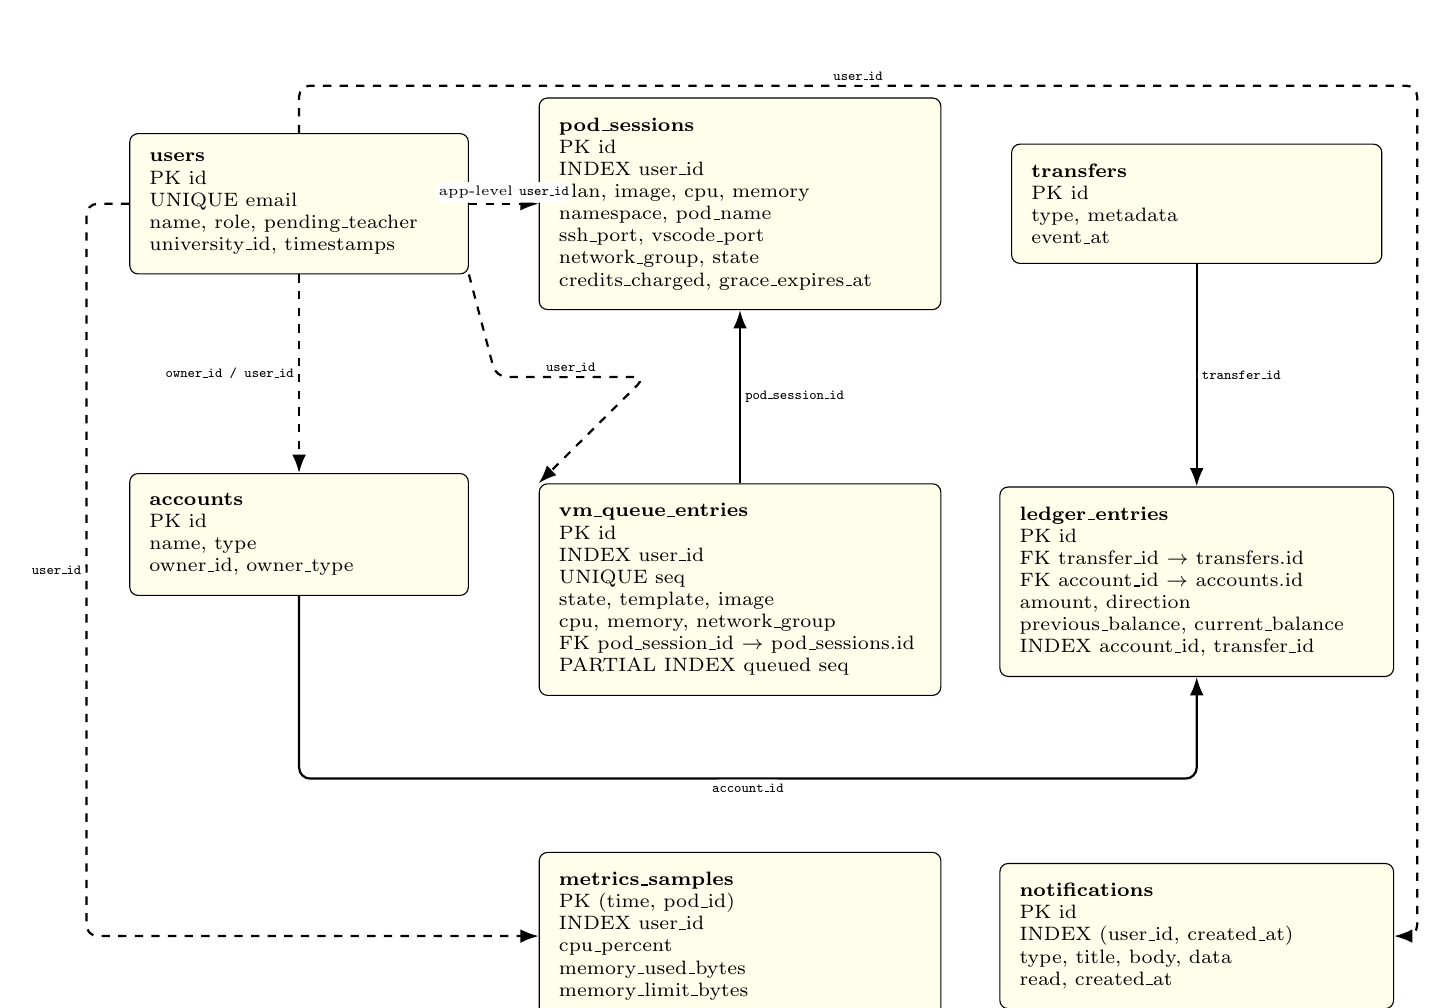
\begin{tikzpicture}[
    font=\scriptsize,
    >=Latex,
    entity/.style={
        draw,
        rounded corners=3pt,
        align=left,
        fill=yellow!8,
        inner sep=2.5mm
    },
    rel/.style={
        ->,
        thick,
        rounded corners=4pt
    },
    apprel/.style={
        ->,
        thick,
        dashed,
        rounded corners=4pt
    },
    edgeLabel/.style={
        font=\tiny,
        fill=white,
        inner sep=1.5pt,
        align=center
    }
]

% Left column
\node[entity, text width=38mm] (users) at (0,0) {
    \textbf{users}\\
    PK id\\
    UNIQUE email\\
    name, role, pending\_teacher\\
    university\_id, timestamps
};

\node[entity, text width=38mm] (accounts) at (0,-4.2) {
    \textbf{accounts}\\
    PK id\\
    name, type\\
    owner\_id, owner\_type
};

% Centre column
\node[entity, text width=46mm] (sessions) at (5.6,0) {
    \textbf{pod\_sessions}\\
    PK id\\
    INDEX user\_id\\
    plan, image, cpu, memory\\
    namespace, pod\_name\\
    ssh\_port, vscode\_port\\
    network\_group, state\\
    credits\_charged, grace\_expires\_at
};

\node[entity, text width=46mm] (queue) at (5.6,-4.9) {
    \textbf{vm\_queue\_entries}\\
    PK id\\
    INDEX user\_id\\
    UNIQUE seq\\
    state, template, image\\
    cpu, memory, network\_group\\
    FK pod\_session\_id $\rightarrow$ pod\_sessions.id\\
    PARTIAL INDEX queued seq
};

\node[entity, text width=46mm] (metrics) at (5.6,-9.3) {
    \textbf{metrics\_samples}\\
    PK (time, pod\_id)\\
    INDEX user\_id\\
    cpu\_percent\\
    memory\_used\_bytes\\
    memory\_limit\_bytes
};

% Right column
\node[entity, text width=42mm] (transfers) at (11.4,0) {
    \textbf{transfers}\\
    PK id\\
    type, metadata\\
    event\_at
};

\node[entity, text width=45mm] (entries) at (11.4,-4.8) {
    \textbf{ledger\_entries}\\
    PK id\\
    FK transfer\_id $\rightarrow$ transfers.id\\
    FK account\_id $\rightarrow$ accounts.id\\
    amount, direction\\
    previous\_balance, current\_balance\\
    INDEX account\_id, transfer\_id
};

\node[entity, text width=45mm] (notifications) at (11.4,-9.3) {
    \textbf{notifications}\\
    PK id\\
    INDEX (user\_id, created\_at)\\
    type, title, body, data\\
    read, created\_at
};

% Direct relationships
\draw[apprel]
    (users.east)
    --
    node[edgeLabel, above] {app-level \texttt{user\_id}}
    (sessions.west);

\draw[apprel]
    (users.south)
    --
    node[edgeLabel, left] {\texttt{owner\_id / user\_id}}
    (accounts.north);

\draw[rel]
    (queue.north)
    --
    node[edgeLabel, right] {\texttt{pod\_session\_id}}
    (sessions.south);

\draw[rel]
    (transfers.south)
    --
    node[edgeLabel, right] {\texttt{transfer\_id}}
    (entries.north);

% Users to queue, routed through the empty middle gap
\coordinate (userQueueA) at (2.5,-2.2);
\coordinate (userQueueB) at (4.4,-2.2);

\draw[apprel]
    (users.south east)
    --
    (userQueueA)
    --
    node[edgeLabel, above] {\texttt{user\_id}}
    (userQueueB)
    --
    (queue.north west);

% Accounts to ledger entries, routed below the middle row
\coordinate (accountEntryA) at (0,-7.3);
\coordinate (accountEntryB) at (11.4,-7.3);

\draw[rel]
    (accounts.south)
    --
    (accountEntryA)
    --
    node[edgeLabel, below] {\texttt{account\_id}}
    (accountEntryB)
    --
    (entries.south);

% Users to metrics, routed outside the left edge
\coordinate (metricsRouteA) at (-2.7,0);
\coordinate (metricsRouteB) at (-2.7,-9.3);

\draw[apprel]
    (users.west)
    --
    (metricsRouteA)
    --
    node[edgeLabel, left] {\texttt{user\_id}}
    (metricsRouteB)
    --
    (metrics.west);

% Users to notifications, routed outside the top and right edges
\coordinate (notifyRouteA) at (0,1.5);
\coordinate (notifyRouteB) at (14.2,1.5);
\coordinate (notifyRouteC) at (14.2,-9.3);

\draw[apprel]
    (users.north)
    --
    (notifyRouteA)
    --
    node[edgeLabel, above] {\texttt{user\_id}}
    (notifyRouteB)
    --
    (notifyRouteC)
    --
    (notifications.east);

\end{tikzpicture}}
    \caption{Core entity relationships derived from SQLAlchemy models and Alembic migrations. Solid arrows indicate database-enforced foreign keys; dashed arrows indicate application-level links stored by identifier only.}
    \label{fig:hopper-core-erd}
\end{figure}

Figure~\ref{fig:hopper-core-erd} highlights an important characteristic of the current schema: not every logical relationship is enforced with a foreign key. The strongest database-enforced relationships are in the credit ledger, where \texttt{ledger\_entries.transfer\_id} references \texttt{transfers.id}, \texttt{ledger\_entries.account\_id} references \texttt{accounts.id}, and \texttt{vm\_queue\_entries.pod\_session\_id} references \texttt{pod\_sessions.id}. By contrast, many user-owned records such as \texttt{pod\_sessions}, \texttt{notifications}, and \texttt{api\_keys} store a \texttt{user\_id} without a declared SQL foreign key. Ownership is therefore enforced primarily through application logic and authenticated route checks rather than through a dense relational constraint graph.

The credit subsystem is intentionally normalized into three tables: \texttt{accounts}, \texttt{transfers}, and \texttt{ledger\_entries}. This supports double-entry accounting and avoids storing mutable balances as the only source of truth. The initial migration also creates indexes on \texttt{ledger\_entries.account\_id} and \texttt{ledger\_entries.transfer\_id} and uses PostgreSQL rules to prevent updates or deletes on ledger rows and transfers. That design decision is consistent with the service code, which treats the ledger as append-only and uses transaction-level locking to serialize deductions.

The VM lifecycle subsystem centers on \texttt{pod\_sessions}. Each row stores the user-facing VM identity, selected plan, image, CPU and memory limits, namespace and pod name, exposed ports, current state, accumulated credits, and optional network-group data. Queueing is separated into \texttt{vm\_queue\_entries}, which freezes the requested plan and resolved image at enqueue time and adds a monotonically increasing \texttt{seq} field. The migration creating this table also defines a partial index on queued rows by sequence, which supports efficient first-come, first-served head-of-line admission scans.

The notification and metrics subsystems are also specialized rather than overloaded into a generic event table. Notifications form a rolling per-user window backed by a composite index on \texttt{(user\_id, created\_at)} because the main queries are recent notifications and unread counts. Metrics are stored in \texttt{metrics\_samples} with a composite primary key \texttt{(time, pod\_id)} and a separate index on \texttt{user\_id}. The migration attempts to create a Timescale hypertable and retention policy when the database supports those functions, but it explicitly degrades gracefully to a regular PostgreSQL table when TimescaleDB is unavailable.

Several auxiliary tables exist outside the core ERD and contribute to operational completeness: \texttt{audit\_logs}, \texttt{ssh\_keys}, \texttt{issue\_reports}, \texttt{email\_codes}, \texttt{scheduler\_leader}, and \texttt{api\_keys}. These support auditing, SSH management, issue reporting, email verification and reset flows, leader election for the scheduler loop, and scoped programmatic access. Because Section 2 focuses on the main architectural data paths, they are described here textually rather than all being included in one overloaded ERD figure.

\begin{figure}[H]
    \centering
    \resizebox{\textwidth}{!}{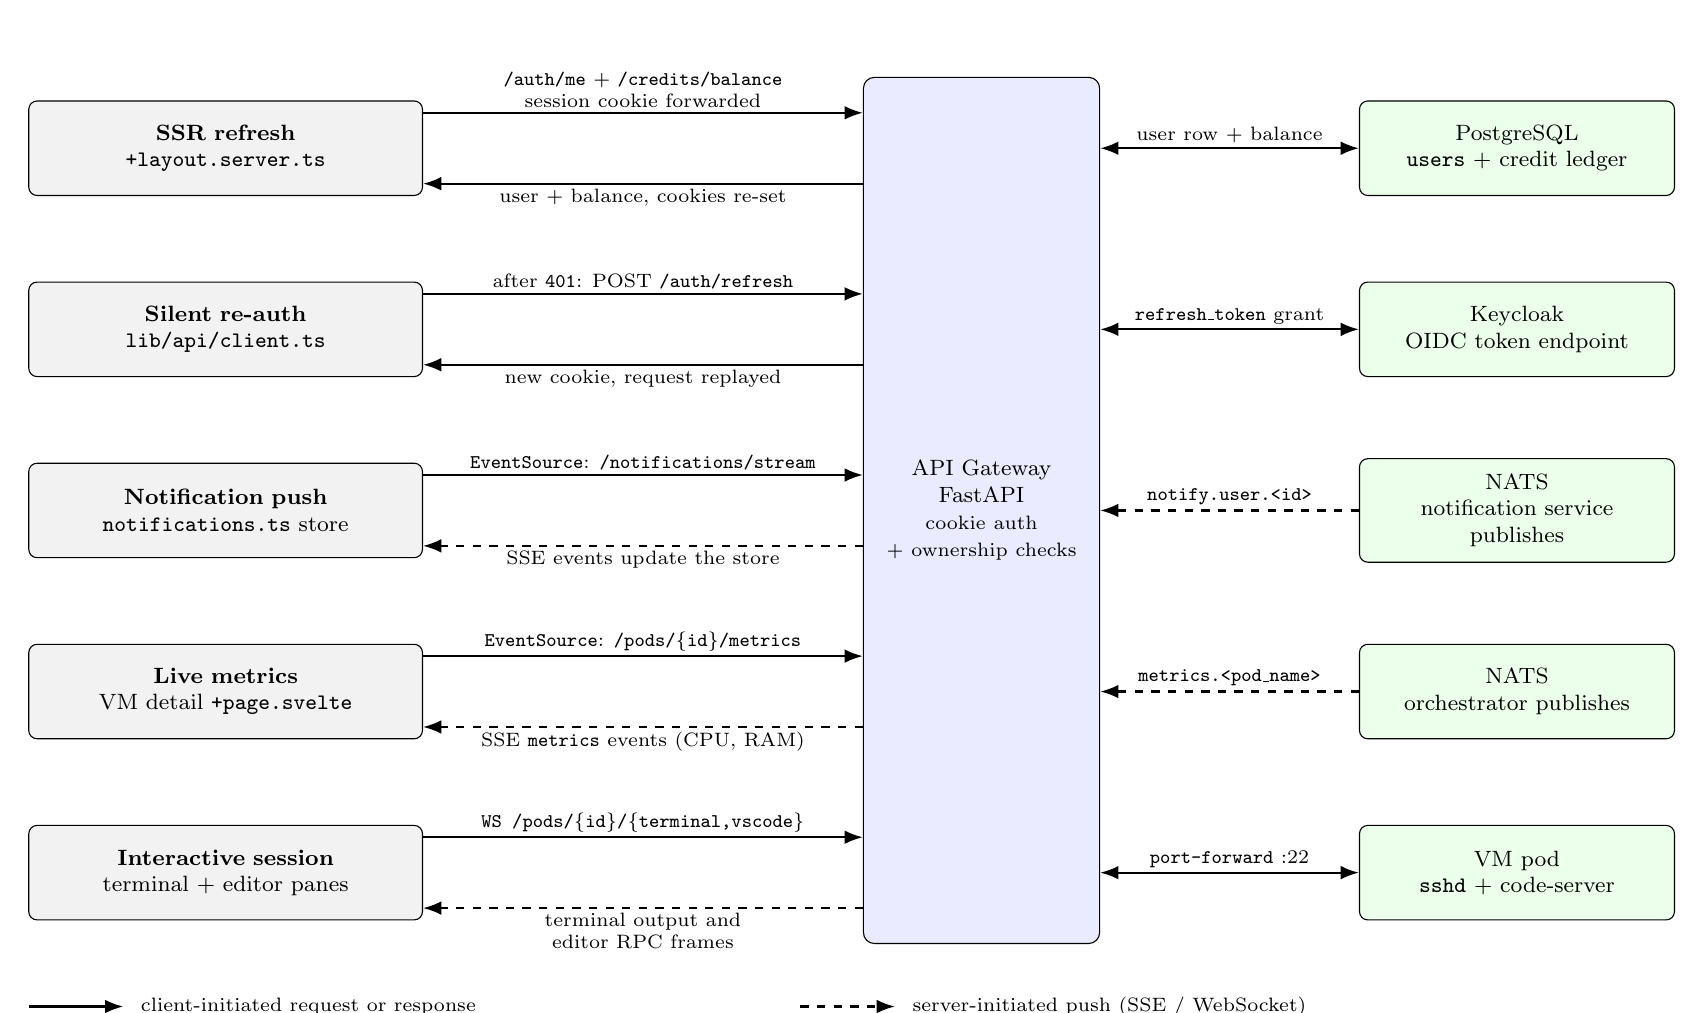
\begin{tikzpicture}[
    font=\footnotesize,
    >=Latex,
    client/.style={
        draw,
        rounded corners=3pt,
        align=center,
        text width=46mm,
        minimum height=12mm,
        inner sep=2mm,
        fill=gray!10
    },
    backend/.style={
        draw,
        rounded corners=3pt,
        align=center,
        text width=36mm,
        minimum height=12mm,
        inner sep=2mm,
        fill=green!8
    },
    gateway/.style={
        draw,
        rounded corners=4pt,
        align=center,
        text width=26mm,
        minimum width=30mm,
        minimum height=110mm,
        inner sep=2mm,
        fill=blue!8
    },
    req/.style={
        ->,
        thick
    },
    push/.style={
        ->,
        thick,
        dashed
    },
    both/.style={
        <->,
        thick
    },
    lab/.style={
        font=\scriptsize,
        fill=white,
        inner sep=1.5pt,
        align=center
    }
]

% Middle spine: the single API gateway shared by every sync mechanism
\node[gateway] (gw) at (9.6,-4.6)
    {API Gateway\\FastAPI\\[2pt]\scriptsize cookie auth\\\scriptsize + ownership checks};


% Lane 1 --- server-rendered refresh of auth state and balance
\node[client]  (c1) at (0,0)
    {\textbf{SSR refresh}\\\texttt{+layout.server.ts}};
\node[backend] (b1) at (16.4,0)
    {PostgreSQL\\\texttt{users} + credit ledger};

\draw[req]
    ($(c1.east)+(0,0.45)$)
    --
    node[lab, above] {\texttt{/auth/me} + \texttt{/credits/balance}\\session cookie forwarded}
    ($(gw.west |- c1.east)+(0,0.45)$);

\draw[req]
    ($(gw.west |- c1.east)-(0,0.45)$)
    --
    node[lab, below] {user + balance, cookies re-set}
    ($(c1.east)-(0,0.45)$);

\draw[both]
    (gw.east |- b1.west)
    --
    node[lab, above] {user row + balance}
    (b1.west);


% Lane 2 --- browser-side silent token refresh and replay
\node[client]  (c2) at (0,-2.3)
    {\textbf{Silent re-auth}\\\texttt{lib/api/client.ts}};
\node[backend] (b2) at (16.4,-2.3)
    {Keycloak\\OIDC token endpoint};

\draw[req]
    ($(c2.east)+(0,0.45)$)
    --
    node[lab, above] {after \texttt{401}: POST \texttt{/auth/refresh}}
    ($(gw.west |- c2.east)+(0,0.45)$);

\draw[req]
    ($(gw.west |- c2.east)-(0,0.45)$)
    --
    node[lab, below] {new cookie, request replayed}
    ($(c2.east)-(0,0.45)$);

\draw[both]
    (gw.east |- b2.west)
    --
    node[lab, above] {\texttt{refresh\_token} grant}
    (b2.west);


% Lane 3 --- notification fan-out over SSE
\node[client]  (c3) at (0,-4.6)
    {\textbf{Notification push}\\\texttt{notifications.ts} store};
\node[backend] (b3) at (16.4,-4.6)
    {NATS\\notification service\\publishes};

\draw[req]
    ($(c3.east)+(0,0.45)$)
    --
    node[lab, above] {\texttt{EventSource}: \texttt{/notifications/stream}}
    ($(gw.west |- c3.east)+(0,0.45)$);

\draw[push]
    ($(gw.west |- c3.east)-(0,0.45)$)
    --
    node[lab, below] {SSE events update the store}
    ($(c3.east)-(0,0.45)$);

\draw[push]
    (b3.west)
    --
    node[lab, above] {\texttt{notify.user.<id>}}
    (gw.east |- b3.west);


% Lane 4 --- live pod metrics over a separate SSE stream
\node[client]  (c4) at (0,-6.9)
    {\textbf{Live metrics}\\VM detail \texttt{+page.svelte}};
\node[backend] (b4) at (16.4,-6.9)
    {NATS\\orchestrator publishes};

\draw[req]
    ($(c4.east)+(0,0.45)$)
    --
    node[lab, above] {\texttt{EventSource}: \texttt{/pods/\{id\}/metrics}}
    ($(gw.west |- c4.east)+(0,0.45)$);

\draw[push]
    ($(gw.west |- c4.east)-(0,0.45)$)
    --
    node[lab, below] {SSE \texttt{metrics} events (CPU, RAM)}
    ($(c4.east)-(0,0.45)$);

\draw[push]
    (b4.west)
    --
    node[lab, above] {\texttt{metrics.<pod\_name>}}
    (gw.east |- b4.west);


% Lane 5 --- interactive sessions bridged through the gateway
\node[client]  (c5) at (0,-9.2)
    {\textbf{Interactive session}\\terminal + editor panes};
\node[backend] (b5) at (16.4,-9.2)
    {VM pod\\\texttt{sshd} + code-server};

\draw[req]
    ($(c5.east)+(0,0.45)$)
    --
    node[lab, above] {\texttt{WS /pods/\{id\}/\{terminal,vscode\}}}
    ($(gw.west |- c5.east)+(0,0.45)$);

\draw[push]
    ($(gw.west |- c5.east)-(0,0.45)$)
    --
    node[lab, below] {terminal output and\\editor RPC frames}
    ($(c5.east)-(0,0.45)$);

\draw[both]
    (gw.east |- b5.west)
    --
    node[lab, above] {\texttt{port-forward} :22}
    (b5.west);


% Legend
\draw[req] (-2.5,-10.9) -- (-1.3,-10.9);
\node[font=\scriptsize, anchor=west] at (-1.2,-10.9)
    {client-initiated request or response};

\draw[push] (7.3,-10.9) -- (8.5,-10.9);
\node[font=\scriptsize, anchor=west] at (8.6,-10.9)
    {server-initiated push (SSE / WebSocket)};

\end{tikzpicture}
}
    \caption{Verified automatic UI data-sync mechanisms: SSR refresh, SSE streams, and WebSocket proxying.}
    \label{fig:hopper-ui-sync}
\end{figure}

The repository confirms that automatic UI synchronization is implemented in multiple ways rather than through one generic push channel. As shown in Figure~\ref{fig:hopper-ui-sync}, the layout loader refreshes authentication state and forwards cookies server-side, the browser-side API client retries after silent refresh on eligible \texttt{401} responses, notifications are pushed over an \texttt{EventSource} stream, pod metrics are streamed through a separate \texttt{EventSource}, and terminal or browser-based editor access is proxied through WebSocket or HTTP upgrade paths in the gateway. This is a concrete, code-backed real-time strategy. It should therefore be documented as a combination of SSR data refresh, SSE fan-out, and backend-mediated interactive proxies rather than as a generic polling-only or WebSocket-only system.

\section{API Documentation}
\subsection{API Design Overview}
Hopper exposes a primarily REST-style HTTP API through the FastAPI gateway in \path|services/api-gateway/app/main.py|. The frontend API client hard-codes \path|/api| as its public base path, and the Kubernetes ingress rewrites that path before forwarding requests to the gateway service. Internally, the application routers are mounted directly at prefixes such as \path|/auth|, \path|/pods|, \path|/credits|, and \path|/admin|; externally, users reach them as \path|/api/auth|, \path|/api/pods|, \path|/api/credits|, and so on. The application metadata declares API version \texttt{0.1.0}, but the repository does not implement URI-based versioning such as \path|/v1|. The current versioning approach is therefore documentation-level rather than path-level.

The dominant request and response format is JSON over HTTPS. FastAPI and Pydantic models are used for request validation and typed response shaping, for example \path|LoginRequest|, \path|SignupRequest|, \path|CreatePodRequest|, \path|PodResponse|, \path|CreditBalanceResponse|, and \path|UserResponse|. The frontend client sets \texttt{Content-Type: application/json} automatically for non-form submissions and includes browser credentials on every request. A smaller set of endpoints uses alternative transports where the feature requires them: file upload uses \texttt{multipart/form-data}, file download returns \texttt{application/octet-stream}, notification and metrics feeds use Server-Sent Events (SSE), and terminal or browser-editor sessions use proxied WebSocket or HTTP upgrade paths.

Authentication is enforced through the shared dependency \path|get_current_user()|. The main browser flow uses secure HttpOnly cookies, especially \path|session_token| and \path|refresh_token|, which are issued after successful Keycloak-backed sign-in. Programmatic access is also supported through Hopper API keys supplied either in \texttt{X-API-Key} or as \texttt{Authorization: Bearer hop\_...}. The code explicitly restricts \texttt{read\_only} API keys to \texttt{GET}, \texttt{HEAD}, and \texttt{OPTIONS} requests, while API-key creation and revocation require a real cookie-backed session. Authorization is role-aware rather than endpoint-global: the repository verifies at least three roles, namely \texttt{student}, \texttt{professor}, and \texttt{admin}.

Validation and error handling are a combination of schema validation and route-level checks. Pydantic enforces field structure, lengths, and constrained values, while the routers enforce application rules such as credit sufficiency, ownership, allowed domains, password policy, and role restrictions. The common error format is FastAPI's JSON \texttt{\{"detail": "..."\}} payload, although validation failures inherited from framework-level schema errors may return the standard structured \texttt{422} detail list. The codebase also shows consistent use of meaningful HTTP status codes such as \texttt{201 Created}, \texttt{202 Accepted}, \texttt{204 No Content}, \texttt{401 Unauthorized}, \texttt{402 Payment Required}, \texttt{403 Forbidden}, \texttt{404 Not Found}, \texttt{409 Conflict}, \texttt{422 Unprocessable Entity}, and \texttt{429 Too Many Requests}.

The API does not follow one universal pagination contract, but several repeatable conventions are implemented. Credit history and audit-log style listings use \path|limit| and \path|offset| query parameters. Notification and issue listing endpoints impose bounded maximums, and issue administration accepts a simple \path|status| filter. Usage endpoints accept a \path|range| parameter with confirmed values \path|1h|, \path|6h|, \path|24h|, and \path|7d| to control aggregation windows. These conventions are pragmatic and code-backed, but they are not wrapped in a separate global pagination abstraction at the current stage of the project.

\subsection{Endpoint Reference}
The report focuses on the important public application endpoints that are intended for user-facing or evaluator-facing interaction. Internal readiness and liveness handlers such as \path|/healthz| and \path|/readyz| are deliberately excluded from the main table because they are deployment-facing operational probes rather than end-user APIs.

\textbf{Authentication and identity endpoints}

\begingroup
\scriptsize
\setlength{\tabcolsep}{4pt}
\begin{longtable}{|>{\RaggedRight\arraybackslash}p{0.10\textwidth}|>{\RaggedRight\arraybackslash}p{0.23\textwidth}|>{\RaggedRight\arraybackslash}p{0.26\textwidth}|>{\RaggedRight\arraybackslash}p{0.12\textwidth}|>{\RaggedRight\arraybackslash}p{0.14\textwidth}|}
    \hline
    \textbf{Method} & \textbf{Route} & \textbf{Purpose} & \textbf{Auth} & \textbf{Authorized Role} \\
    \hline
    \endfirsthead
    \hline
    \textbf{Method} & \textbf{Route} & \textbf{Purpose} & \textbf{Auth} & \textbf{Authorized Role} \\
    \hline
    \endhead
    GET & \path|/api/auth/login| & Starts the OIDC login flow with PKCE, state, and nonce, then redirects the browser to Keycloak. & No & Public \\
    \hline
    POST & \path|/api/auth/signup| & Creates a local-account sign-up request with role selection and password-policy checks. & No & Public \\
    \hline
    POST & \path|/api/auth/verify-email| & Confirms an emailed verification code. & No & Public \\
    \hline
    POST & \path|/api/auth/resend-code| & Re-sends a verification or password-reset code. & No & Public \\
    \hline
    POST & \path|/api/auth/forgot-password| & Starts the password-reset flow for an existing account email. & No & Public \\
    \hline
    POST & \path|/api/auth/reset-password| & Resets a password after code validation and, where applicable, marks the email verified. & No & Public \\
    \hline
    POST & \path|/api/auth/login| & Performs direct email-password login and issues session cookies on success. & No & Public \\
    \hline
    GET & \path|/api/auth/callback| & Completes the OIDC authorization-code exchange after Keycloak redirects back. & No & Public callback endpoint \\
    \hline
    POST & \path|/api/auth/refresh| & Uses the refresh-token cookie to mint a new access cookie. & Refresh cookie & Session holder \\
    \hline
    GET & \path|/api/auth/me| & Returns the authenticated user's current profile and pending-teacher status. & Yes & Any authenticated user \\
    \hline
    POST & \path|/api/auth/logout| & Revokes the refresh token where possible, clears cookies, and redirects to Keycloak logout. & Yes & Any authenticated user \\
    \hline
    POST & \path|/api/auth/api-keys| & Creates an API key and returns the plaintext key exactly once. & Yes & Any authenticated user with session cookie \\
    \hline
    GET & \path|/api/auth/api-keys| & Lists the caller's API keys without revealing stored secrets. & Yes & Any authenticated user \\
    \hline
    DELETE & \path|/api/auth/api-keys/\{key\_id\}| & Revokes one of the caller's API keys. & Yes & Any authenticated user with session cookie \\
    \hline
\end{longtable}
\endgroup

\textbf{Pod lifecycle and interactive session endpoints}

\begingroup
\scriptsize
\setlength{\tabcolsep}{4pt}
\begin{longtable}{|>{\RaggedRight\arraybackslash}p{0.10\textwidth}|>{\RaggedRight\arraybackslash}p{0.23\textwidth}|>{\RaggedRight\arraybackslash}p{0.26\textwidth}|>{\RaggedRight\arraybackslash}p{0.12\textwidth}|>{\RaggedRight\arraybackslash}p{0.14\textwidth}|}
    \hline
    \textbf{Method} & \textbf{Route} & \textbf{Purpose} & \textbf{Auth} & \textbf{Authorized Role} \\
    \hline
    \endfirsthead
    \hline
    \textbf{Method} & \textbf{Route} & \textbf{Purpose} & \textbf{Auth} & \textbf{Authorized Role} \\
    \hline
    \endhead
    GET & \path|/api/pods/plans| & Returns the plan catalogue exposed to the provisioning UI. & No & Public \\
    \hline
    GET & \path|/api/pods/| & Lists the current user's pod sessions. & Yes & Any authenticated user \\
    \hline
    POST & \path|/api/pods/| & Creates a pod synchronously when capacity is available, or returns \texttt{202 Accepted} with queue information when the request is enqueued. & Yes & Any authenticated user; \path|network_group| limited to professor/admin \\
    \hline
    GET & \path|/api/pods/availability| & Reports whether synchronous capacity is currently available together with queue length. & Yes & Any authenticated user \\
    \hline
    GET & \path|/api/pods/queue| & Lists the caller's active queue entries and queue positions. & Yes & Any authenticated user \\
    \hline
    DELETE & \path|/api/pods/queue/\{entry\_id\}| & Cancels one of the caller's still-queued VM requests. & Yes & Queue-entry owner \\
    \hline
    GET & \path|/api/pods/\{pod\_id\}| & Returns details of a specific pod session. & Yes & Pod owner \\
    \hline
    DELETE & \path|/api/pods/\{pod\_id\}| & Terminates a pod session and releases its reserved resources. & Yes & Pod owner \\
    \hline
    GET & \path|/api/pods/\{pod\_id\}/metrics| & Streams live pod metrics to the UI through Server-Sent Events. & Yes & Pod owner \\
    \hline
    HTTP proxy & \path|/api/pods/\{pod\_id\}/vscode/\{path\}| & Proxies browser-based code-server traffic for an owned pod across \texttt{GET}, \texttt{POST}, \texttt{PUT}, \texttt{PATCH}, \texttt{DELETE}, and \texttt{OPTIONS}. & Yes & Pod owner \\
    \hline
    WS & \path|/api/pods/\{pod\_id\}/vscode/\{path\}| & WebSocket upgrade path used by the proxied browser editor. & Yes & Pod owner \\
    \hline
    WS & \path|/api/pods/\{pod\_id\}/terminal| & Provides interactive terminal access to a running pod. & Yes & Pod owner \\
    \hline
\end{longtable}
\endgroup

\textbf{Credits and usage endpoints}

\begingroup
\scriptsize
\setlength{\tabcolsep}{4pt}
\begin{longtable}{|>{\RaggedRight\arraybackslash}p{0.10\textwidth}|>{\RaggedRight\arraybackslash}p{0.23\textwidth}|>{\RaggedRight\arraybackslash}p{0.26\textwidth}|>{\RaggedRight\arraybackslash}p{0.12\textwidth}|>{\RaggedRight\arraybackslash}p{0.14\textwidth}|}
    \hline
    \textbf{Method} & \textbf{Route} & \textbf{Purpose} & \textbf{Auth} & \textbf{Authorized Role} \\
    \hline
    \endfirsthead
    \hline
    \textbf{Method} & \textbf{Route} & \textbf{Purpose} & \textbf{Auth} & \textbf{Authorized Role} \\
    \hline
    \endhead
    GET & \path|/api/credits/balance| & Returns the caller's current credit balance and account identifier. & Yes & Any authenticated user \\
    \hline
    GET & \path|/api/credits/history?limit=\dots\&offset=\dots| & Returns the caller's credit ledger history using limit-offset pagination. & Yes & Any authenticated user \\
    \hline
    GET & \path|/api/credits/teachers| & Lists professor accounts with balances for the admin grant workflow. & Yes & Admin only \\
    \hline
    GET & \path|/api/credits/students| & Lists student accounts with balances for allocation workflows. & Yes & Admin or professor \\
    \hline
    POST & \path|/api/credits/allocate| & Grants or reallocates credits, with semantics that differ for admin and professor roles. & Yes & Admin or professor \\
    \hline
    GET & \path|/api/usage/\{pod\_id\}?range=1h\textbar6h\textbar24h\textbar7d| & Returns historical usage series for a specific pod. & Yes & Any authenticated user \\
    \hline
    GET & \path|/api/usage/summary/me/series?range=1h\textbar6h\textbar24h\textbar7d| & Returns aggregated historical usage across all of the caller's pods. & Yes & Any authenticated user \\
    \hline
    GET & \path|/api/usage/summary/me| & Returns a recent usage summary for the caller. & Yes & Any authenticated user \\
    \hline
\end{longtable}
\endgroup

\textbf{Administration endpoints}

\begingroup
\scriptsize
\setlength{\tabcolsep}{4pt}
\begin{longtable}{|>{\RaggedRight\arraybackslash}p{0.10\textwidth}|>{\RaggedRight\arraybackslash}p{0.23\textwidth}|>{\RaggedRight\arraybackslash}p{0.26\textwidth}|>{\RaggedRight\arraybackslash}p{0.12\textwidth}|>{\RaggedRight\arraybackslash}p{0.14\textwidth}|}
    \hline
    \textbf{Method} & \textbf{Route} & \textbf{Purpose} & \textbf{Auth} & \textbf{Authorized Role} \\
    \hline
    \endfirsthead
    \hline
    \textbf{Method} & \textbf{Route} & \textbf{Purpose} & \textbf{Auth} & \textbf{Authorized Role} \\
    \hline
    \endhead
    GET & \path|/api/admin/users| & Lists all users with role and teacher-approval metadata. & Yes & Admin only \\
    \hline
    GET & \path|/api/admin/teacher-requests| & Lists pending teacher sign-up requests. & Yes & Admin only \\
    \hline
    POST & \path|/api/admin/teacher-requests/\{user\_id\}/approve| & Promotes a pending teacher request to the professor role. & Yes & Admin only \\
    \hline
    POST & \path|/api/admin/teacher-requests/\{user\_id\}/reject| & Rejects a pending teacher request while keeping the user as student. & Yes & Admin only \\
    \hline
    GET & \path|/api/admin/courses| & Returns the current course list. The implementation is presently an empty proof-of-concept response. & Yes & Admin only \\
    \hline
    GET & \path|/api/admin/nodes| & Returns cluster node capacity and readiness data via the orchestrator. & Yes & Admin only \\
    \hline
    GET & \path|/api/admin/stats| & Returns aggregate dashboard statistics such as total users and active VMs. & Yes & Admin only \\
    \hline
    GET & \path|/api/admin/active-vms| & Lists all currently active VM sessions together with owner details. & Yes & Admin only \\
    \hline
    PATCH & \path|/api/admin/users/\{user\_id\}/role| & Changes a user's role with safeguards against invalid or dangerous demotions. & Yes & Admin only \\
    \hline
    GET & \path|/api/admin/audit-logs?limit=\dots\&offset=\dots| & Returns recent audit-log entries using limit-offset pagination. & Yes & Admin only \\
    \hline
\end{longtable}
\endgroup

\textbf{Files, SSH keys, settings, notifications, and issue tracking}

\begingroup
\scriptsize
\setlength{\tabcolsep}{4pt}
\begin{longtable}{|>{\RaggedRight\arraybackslash}p{0.10\textwidth}|>{\RaggedRight\arraybackslash}p{0.23\textwidth}|>{\RaggedRight\arraybackslash}p{0.26\textwidth}|>{\RaggedRight\arraybackslash}p{0.12\textwidth}|>{\RaggedRight\arraybackslash}p{0.14\textwidth}|}
    \hline
    \textbf{Method} & \textbf{Route} & \textbf{Purpose} & \textbf{Auth} & \textbf{Authorized Role} \\
    \hline
    \endfirsthead
    \hline
    \textbf{Method} & \textbf{Route} & \textbf{Purpose} & \textbf{Auth} & \textbf{Authorized Role} \\
    \hline
    \endhead
    PUT & \path|/api/settings/vscode| & Accepts a VS Code settings blob. The current implementation acknowledges the request but still documents future persistence work in comments. & Yes & Any authenticated user \\
    \hline
    GET & \path|/api/ssh-keys/| & Lists the caller's SSH public keys. & Yes & Any authenticated user \\
    \hline
    POST & \path|/api/ssh-keys/| & Adds an SSH public key after format, duplicate, and per-user quota checks. & Yes & Any authenticated user \\
    \hline
    DELETE & \path|/api/ssh-keys/\{key\_id\}| & Deletes one of the caller's SSH keys. & Yes & Key owner \\
    \hline
    GET & \path|/api/files/\{pod\_id\}/list| & Lists files inside a running pod directory. & Yes & Pod owner \\
    \hline
    POST & \path|/api/files/\{pod\_id\}/upload| & Uploads a file to a running pod using multipart form submission and SCP behind the gateway. & Yes & Pod owner \\
    \hline
    GET & \path|/api/files/\{pod\_id\}/download| & Downloads a file from a running pod as an octet-stream attachment. & Yes & Pod owner \\
    \hline
    POST & \path|/api/issues/| & Creates a user issue report, optionally linked to a pod. & Yes & Any authenticated user \\
    \hline
    GET & \path|/api/issues/me| & Lists issue reports submitted by the current user. & Yes & Any authenticated user \\
    \hline
    GET & \path|/api/issues/admin?status=\dots| & Lists issue reports for administrative triage, optionally filtered by status. & Yes & Admin only \\
    \hline
    POST & \path|/api/issues/admin/\{issue\_id\}/resolve| & Marks an issue report as resolved. & Yes & Admin only \\
    \hline
    GET & \path|/api/notifications/| & Returns recent notifications together with an unread count. & Yes & Any authenticated user \\
    \hline
    POST & \path|/api/notifications/read-all| & Marks all of the caller's notifications as read. & Yes & Any authenticated user \\
    \hline
    POST & \path|/api/notifications/\{notification\_id\}/read| & Marks one notification as read. & Yes & Notification owner \\
    \hline
    GET & \path|/api/notifications/stream| & Streams live notifications to the browser using Server-Sent Events. & Yes & Any authenticated user \\
    \hline
\end{longtable}
\endgroup

\subsection{Swagger / Postman Collection Link}
The FastAPI gateway exposes the default Swagger UI, and the repository's ingress configuration makes it reachable publicly at \url{https://hopper.farefin.com/api/docs}. This URL is verified from the combination of the gateway's default FastAPI documentation settings and the ingress rule that forwards the external \path|/api| prefix to the backend service.

No Postman collection URL was found in the inspected repository. The report therefore retains that gap explicitly: \todo{Add a public Postman collection URL if the team publishes one later.}

\subsection{Sample Request \& Response}
\textbf{Example 1: direct login request}

The following example reflects the request body accepted by \path|LoginRequest| in \path|services/api-gateway/app/schemas/user.py|. On success, the handler also sets secure HttpOnly session cookies; those headers are omitted here for brevity and because tokens must not be reproduced in a report.

\begin{lstlisting}[language=bash,caption={Representative login request to the Hopper API}]
curl -X POST "https://hopper.farefin.com/api/auth/login" \
  -H "Content-Type: application/json" \
  -d '{
    "email": "student@example.edu",
    "password": "[REDACTED]"
  }'
\end{lstlisting}

\begin{lstlisting}[caption={Representative login response body}]
{
  "id": "2f3ac4d8-7d3d-4f7b-a2df-0e4f07a8d421",
  "email": "student@example.edu",
  "name": "Example Student",
  "role": "student"
}
\end{lstlisting}

\textbf{Example 2: pod creation request}

This second example shows a provision request based on the verified \path|CreatePodRequest| and \path|PodResponse| schemas. The route may return \texttt{201 Created} for immediate admission or \texttt{202 Accepted} when the request is queued; the JSON below illustrates the immediate-creation path.

\begin{lstlisting}[language=bash,caption={Representative pod creation request}]
curl -X POST "https://hopper.farefin.com/api/pods/" \
  -H "Content-Type: application/json" \
  -H "Cookie: session_token=[REDACTED]" \
  -d '{
    "plan": "small",
    "template": "ubuntu"
  }'
\end{lstlisting}

\begin{lstlisting}[caption={Representative pod creation response body}]
{
  "id": "9bc3d6ee-4b7a-4482-a9de-4948fdde2ce1",
  "user_id": "2f3ac4d8-7d3d-4f7b-a2df-0e4f07a8d421",
  "state": "running",
  "plan": "small",
  "image": "hopper/vm-ubuntu:22.04",
  "cpu": "1",
  "memory": "2Gi",
  "node_name": "worker-1",
  "namespace": "hopper-user-2f3ac4d8",
  "ssh_port": 32022,
  "vscode_port": 32080,
  "ssh_password": "[REDACTED]",
  "network_group": null,
  "created_at": "2026-07-19T12:00:00Z",
  "updated_at": "2026-07-19T12:00:30Z"
}
\end{lstlisting}

\section{Authentication \& Security}
\subsection{Authentication Strategy}
\todo{Describe the verified authentication flow and why it was chosen.}

\subsection{Authorization \& Role Management}
\todo{Document the confirmed application roles and access-control model.}

\subsection{Security Measures}
\todo{Summarize verified validation, secrets handling, rate limiting, network, and transport protections.}

\subsection{Known Vulnerabilities \& Mitigations}
\todo{Add verified known risks, mitigations, and remaining gaps from the repository or test docs.}

\section{Testing \& Quality Assurance}
\subsection{Testing Strategy}
\todo{Summarize the verified unit, integration, end-to-end, and other automated test layers.}

\subsection{Test Coverage Summary}
\todo{Add measured coverage or coverage-report references after verification.}

\subsection{Bug Tracking \& Resolution Log}
\todo{Summarize verified bug-tracking artifacts such as BUG\_TRACKING\_LOG.md.}

\subsection{Sample Test Cases}
\todo{Add representative verified test cases from the current suites.}

\section{CI/CD \& Deployment}
\subsection{Pipeline Overview}
\todo{Describe the verified CI and delivery workflow from repository automation and scripts.}

\subsection{Environments}
\todo{Document the confirmed development, test, staging, and production environments if they exist.}

\subsection{Deployment Steps}
\todo{Summarize the verified deployment procedure from current infrastructure files.}

\subsection{Hosting Platform \& Live URL}
\todo{Add the actual hosting platform and public live URL after verification.}

\subsection{Monitoring \& Logging}
\todo{Describe the verified monitoring, logging, and observability components.}

\section{Repository \& Documentation Quality}
\subsection{Branching Strategy \& Commit Conventions}
\todo{Add the actual branching and commit practices only after verifying repository history or team policy.}

\subsection{README Completeness Checklist}
\todo{Audit the README against setup, environment, run/test, and usage expectations.}

\subsection{Code Organization / Folder Structure}
\todo{Summarize the verified repository structure and service boundaries.}

\subsection{Local Setup Instructions}
\todo{Condense the verified local setup steps for reproducibility.}

\section{Evaluation \& Reflection}
\subsection{Web Performance \& Core Web Vitals}
\todo{Add measured Lighthouse or browser-tool performance metrics later.}

\subsection{Challenges \& Solutions}
\todo{Add verified implementation or deployment challenges and how they were addressed.}

\subsection{Limitations \& Future Work}
\todo{Add realistic limitations and future improvements based on verified project scope.}

\subsection{Lessons Learned}
\todo{Summarize team-level lessons after the full report content is drafted.}

\subsection{Individual Responsibility}
\todo{Replace the placeholder rows with actual team-member responsibilities and contribution evidence.}

\begin{tabularx}{\textwidth}{|>{\RaggedRight\arraybackslash}p{0.17\textwidth}|>{\RaggedRight\arraybackslash}p{0.29\textwidth}|>{\RaggedRight\arraybackslash}X|>{\RaggedRight\arraybackslash}p{0.13\textwidth}|}
    \hline
    \textbf{Member Name} & \textbf{Core Responsibilities \& Feature Ownership} & \textbf{Key PRs / Commit Contributions} & \textbf{Share (\%)} \\
    \hline
    \todo{Add name} & \todo{Add responsibilities} & \todo{Add PRs or commits} & \todo{Add \%} \\
    \hline
    \todo{Add name} & \todo{Add responsibilities} & \todo{Add PRs or commits} & \todo{Add \%} \\
    \hline
    \todo{Add name} & \todo{Add responsibilities} & \todo{Add PRs or commits} & \todo{Add \%} \\
    \hline
    \todo{Add name} & \todo{Add responsibilities} & \todo{Add PRs or commits} & \todo{Add \%} \\
    \hline
    \todo{Add name} & \todo{Add responsibilities} & \todo{Add PRs or commits} & \todo{Add \%} \\
    \hline
    \todo{Add name} & \todo{Add responsibilities} & \todo{Add PRs or commits} & \todo{Add \%} \\
    \hline
    \todo{Add name} & \todo{Add responsibilities} & \todo{Add PRs or commits} & \todo{Add \%} \\
    \hline
    \todo{Add name} & \todo{Add responsibilities} & \todo{Add PRs or commits} & \todo{Add \%} \\
    \hline
\end{tabularx}

\appendix
\section{Screenshots / UI Walkthrough}
\todo{Add annotated screenshots, UI flows, and captions using image files placed under report/figures/.}

\begin{figure}[H]
    \centering
    \fbox{\rule{0pt}{2in}\rule{0.85\textwidth}{0pt}}
    \caption{Placeholder for a UI walkthrough screenshot loaded from \texttt{report/figures/}.}
\end{figure}

\end{document}
